\section{Deployment on Reventador Volcano}
\label{evaluation-sec-deployment}

\begin{figure}[t]
\begin{center}
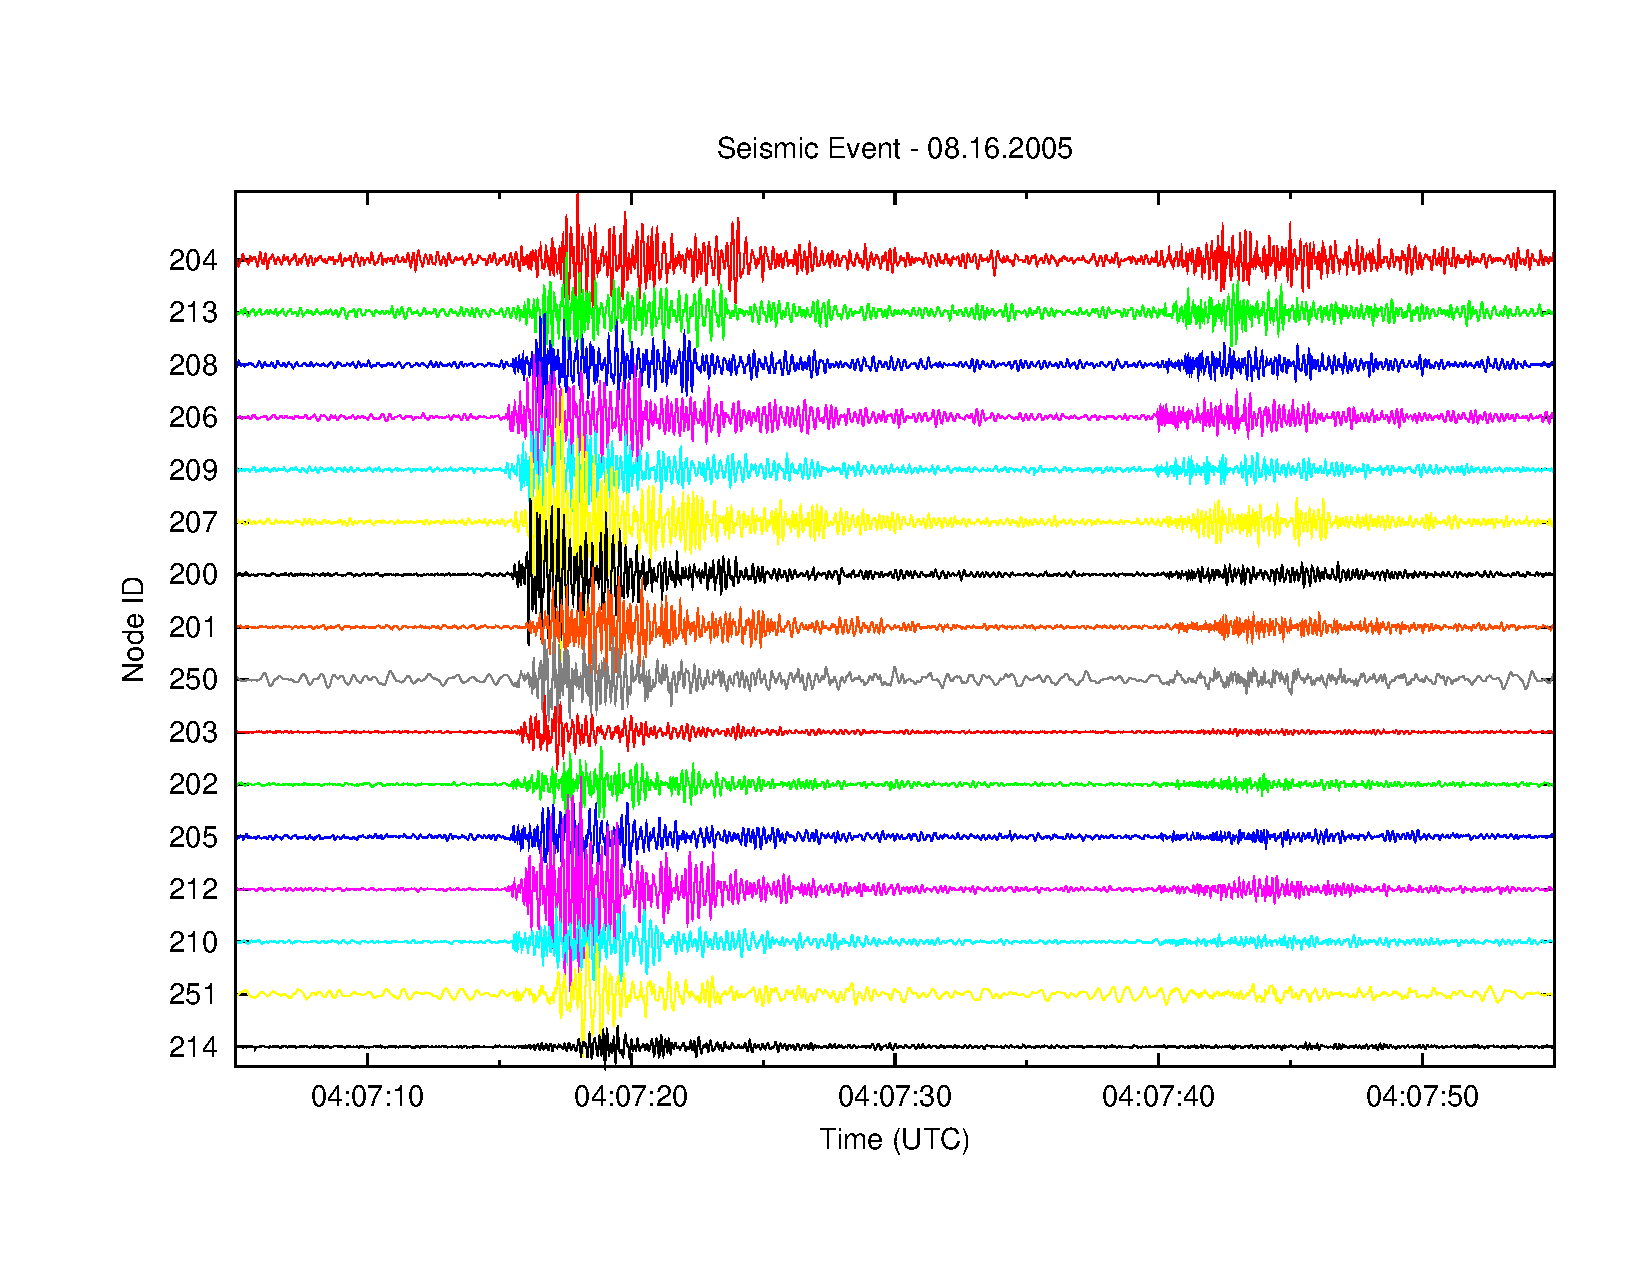
\includegraphics[width=0.7\hsize]{./3-evaluation/figs/event.pdf}
\end{center}
\caption{\textbf{Example of an event captured by our network.} Only seismic
signals are shown. The event shown was a Volcano Tectonic (VT) event and had
no interesting acoustic component. Data shown has undergone several rounds of
post-processing including mapping to GMT time.}
\label{evaluation-fig-event}
\end{figure}

Reventador volcano is located in northern Ecuador, a three hour drive from
the capital, Quito. Long dormant, Reventador reawakened suddenly in 2002,
erupting with massive force. Ash thrown into the air blanketed the streets of
Quito 100~km to the east, closing schools and the airport. Pyroclastic flows
raced down the mountain flattening forests, displacing an oil pipeline, and
severing a major highway. After 18 months of quiescence, renewed activity
began in November 2004.

Our deployment at Reventador took place between August 1--19, 2005. During
this time, Reventador's activity consisted of small explosive events that
ejected ash and incandescent blocks several times a day. Associated
seismicity included numerous explosion earthquakes as well as
extended-duration shaking (tremor) and shallow rock-fracturing earthquakes.

Several features of Reventador made it ideal for our experiment. Reaching
3,500~m at its peak, Reventador sits at a low elevation compared to other
Ecuadorean volcanoes making deployment less strenuous. Its climate is
moderate with temperatures ranging between 10 and 30 degrees Celsius.
Pyroclastic flows produced by the large explosion in 2002 left large parts of
the flanks denuded of vegetation. With the effectiveness of our radio
antennas severely degraded by obstacles to line-of-sight, the lack of
vegetation simplified sensor node positioning.

\begin{figure}[t]
\begin{center}
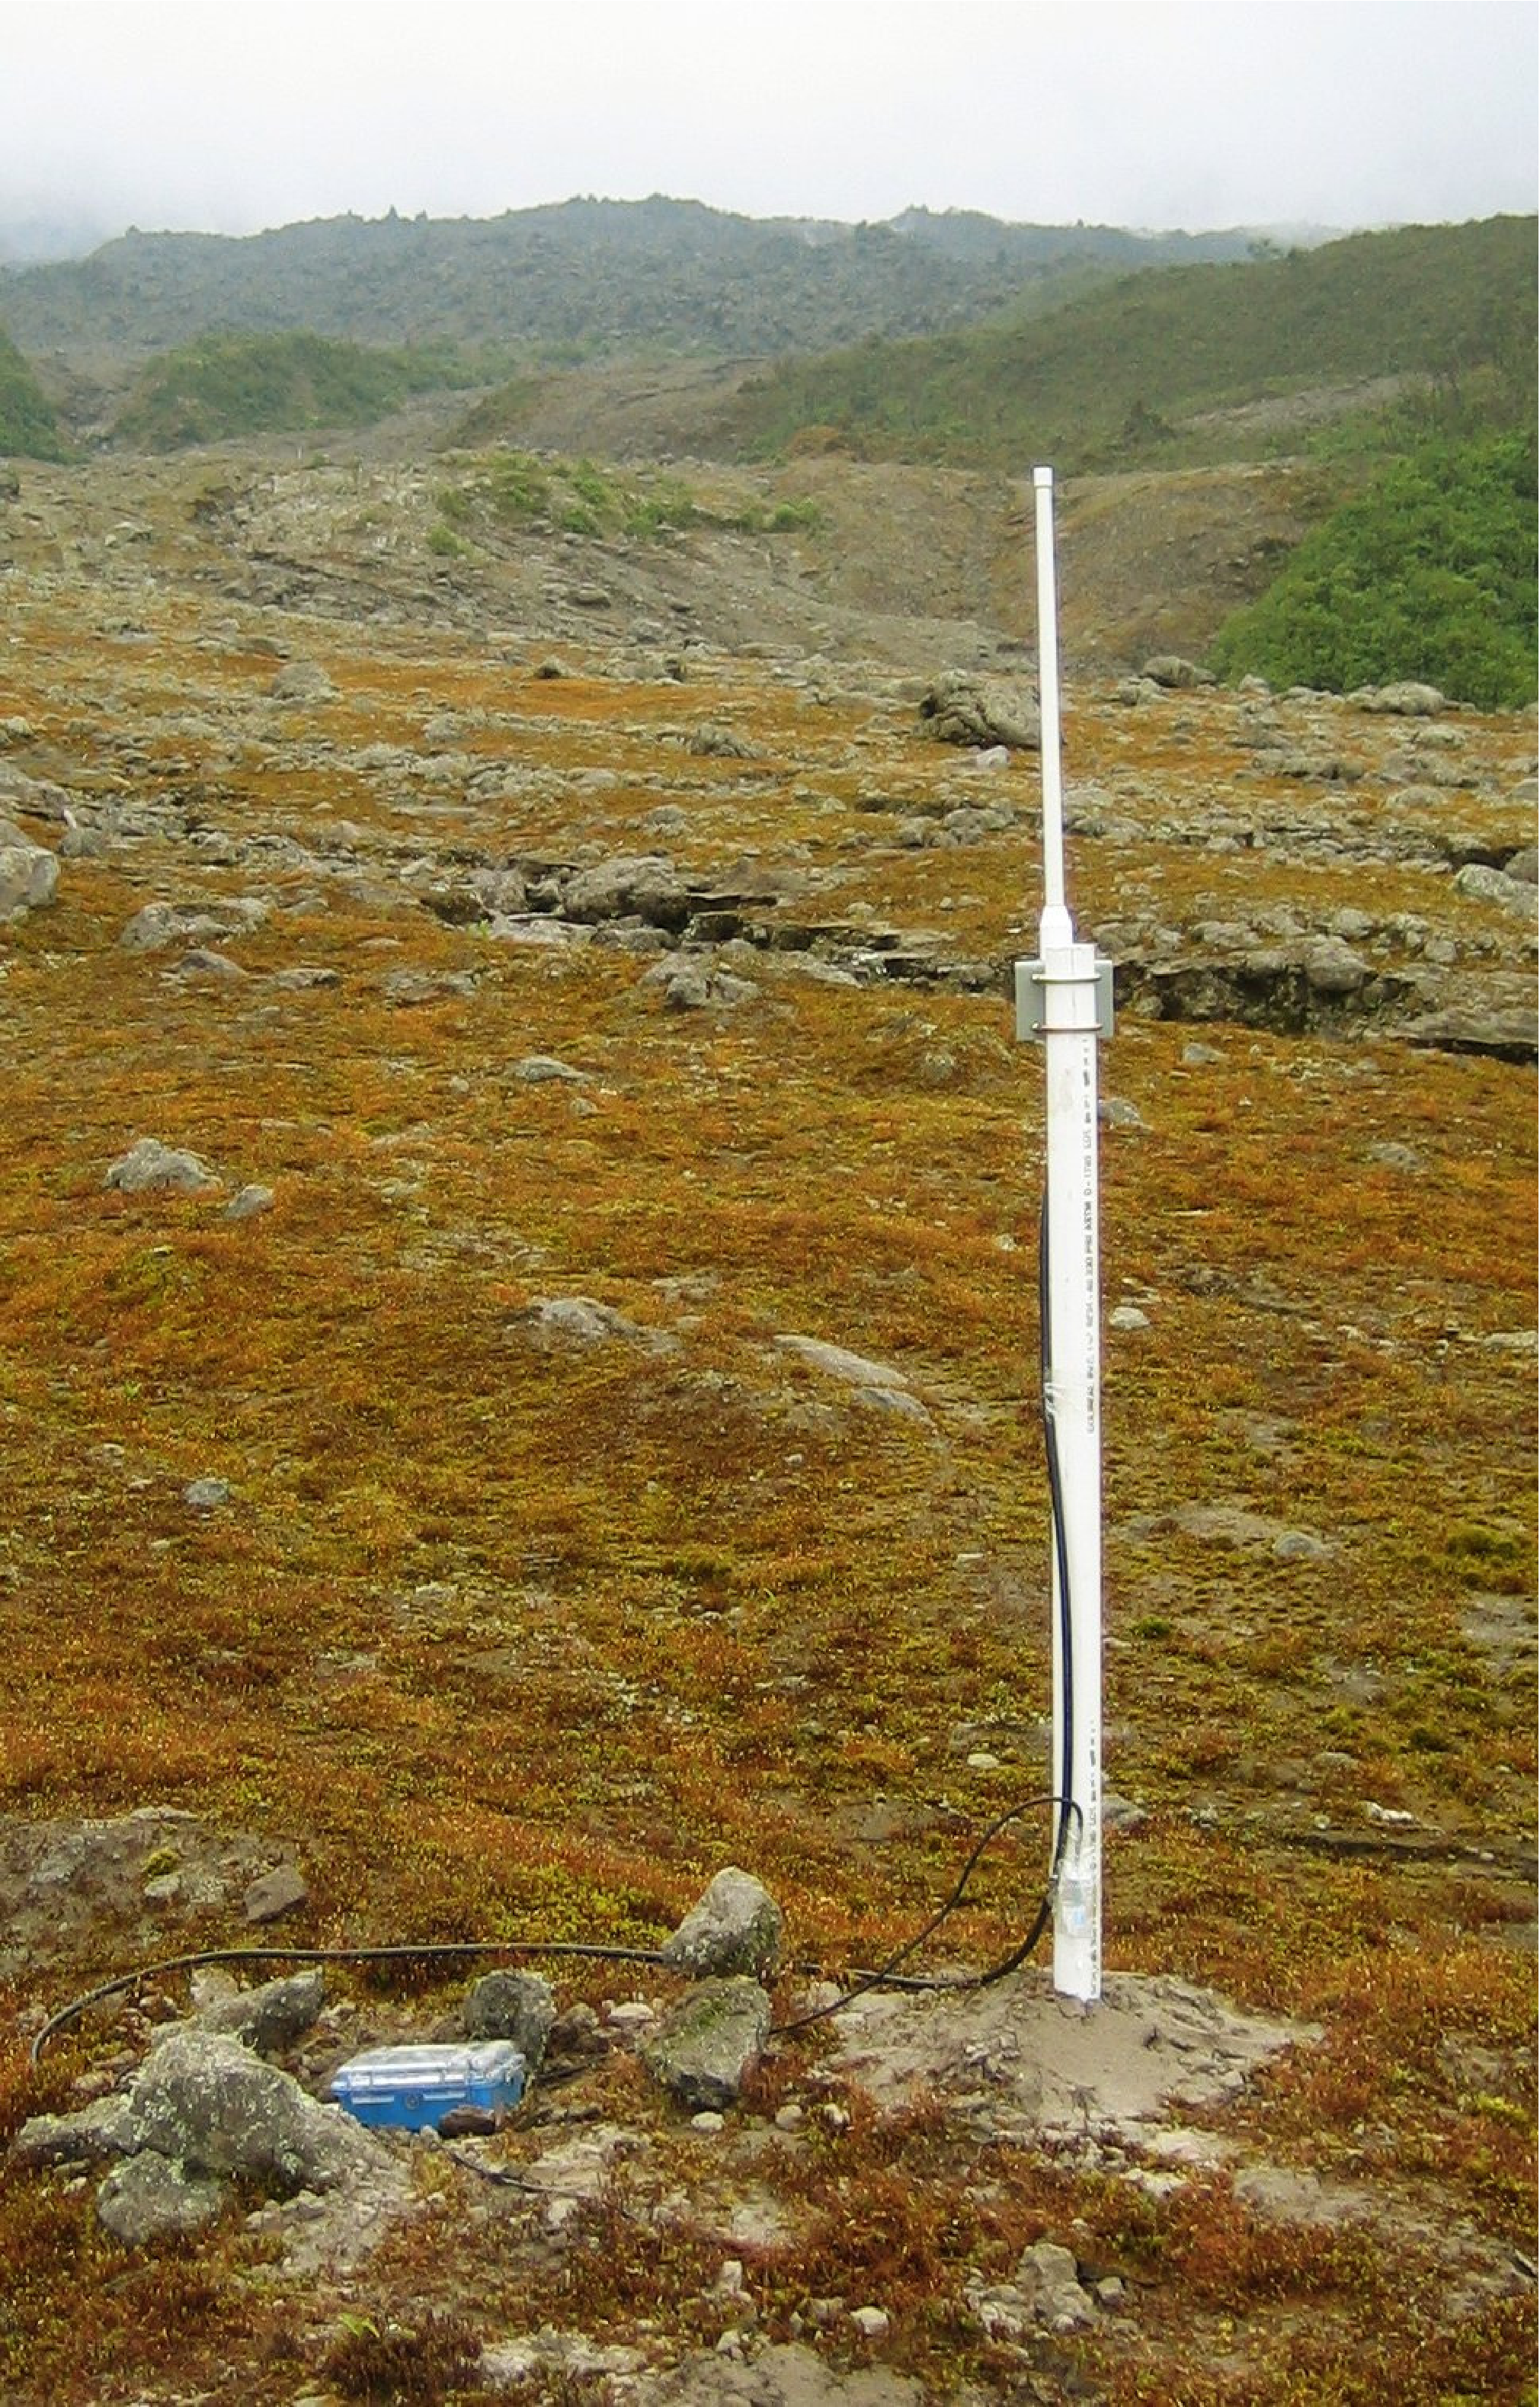
\includegraphics[width=0.5\hsize]{./3-evaluation/figs/station.pdf}
\end{center}
\caption{\textbf{One of our two-component stations.} The blue Pelican Case
contains the wireless sensor network node and hardware interface board. The
external antenna is mounted on the PVC pole to reduce ground effects. A
microphone is taped to the PVC pole and a single seismometer is buried
nearby.}
\label{evaluation-fig-station}
\end{figure}

Our base while working at Reventador was the Hosteria El Reventador, a small
hotel located nearby on the highway from Quito to Lago Agria, about 4.6~km
from the deployment site. The hotel provided us with space to set up our
equipment and ran an electric generator to power our laptops and other
equipment at the makeshift observatory.

The sensors were deployed for a total of 19~days, during which time the
network recorded data from 229~earthquakes, eruptions, and tremor events,
logging 107~MBytes of data. Figure~\ref{evaluation-fig-event} shows data from
a representative event. The long hike and lack of roads prevented frequent
returns to the deployment site, although we returned several times to change
batteries and perform other network maintenance.

\subsection{Sensor Network Device Enclosures and Physical Setup}

A single sensor network node, interface board, and battery holder were all
housed inside a small weatherproof and watertight Pelican case. We installed
environmental connectors through the case allowing cables to external sensors
and antennae to be attached without opening the case and disturbing the
equipment inside. When working in wet and gritty conditions these became a
tremendous asset.

Installing a station involved covering the Pelican case with rocks to anchor
it and shield the contents from direct sunlight. Cables were run from the box
to each sensor and to the antenna. The antenna was elevated on a 1.5~m length
of PVC piping to reduce ground effects which reduce radio range. The
seismometers were buried nearby, but far enough away to remain undisturbed by
any wind-induced shaking of the antenna pole. The microphone was usually
mounted on the antenna pole and shielded from the wind and elements with
plastic tape. Installation took a matter of minutes and the equipment was
sufficiently light and small that six stations could be carried in a large
pack. The PVC poles were light but bulky and proved the most awkward part of
each station to cart around. Figure~\ref{evaluation-fig-station} shows an
example of an installed sensor station.

In addition to the sensor nodes, we used several other pieces of equipment.
Three Freewave~\cite{freewave} radio modems provided a long-distance,
reliable radio link between the sensor network and the observatory laptop.
Freewave modems at the deployment site and the observatory used a 9~dBi
directional Yagi antenna to relay data via a repeater station, installed on a
hill with good line-of-sight to both endpoints. Each Freewave required a car
battery for power, recharged by solar panels. A small number of Crossbow
MicaZ~\cite{micaz} sensor network nodes served in supporting roles. One
interfaced between the network and the Freewave modem; another was attached
to a GPS receiver to provide a global timebase.

\subsection{Network Location and Topology}

\begin{figure}[t]
\begin{center}
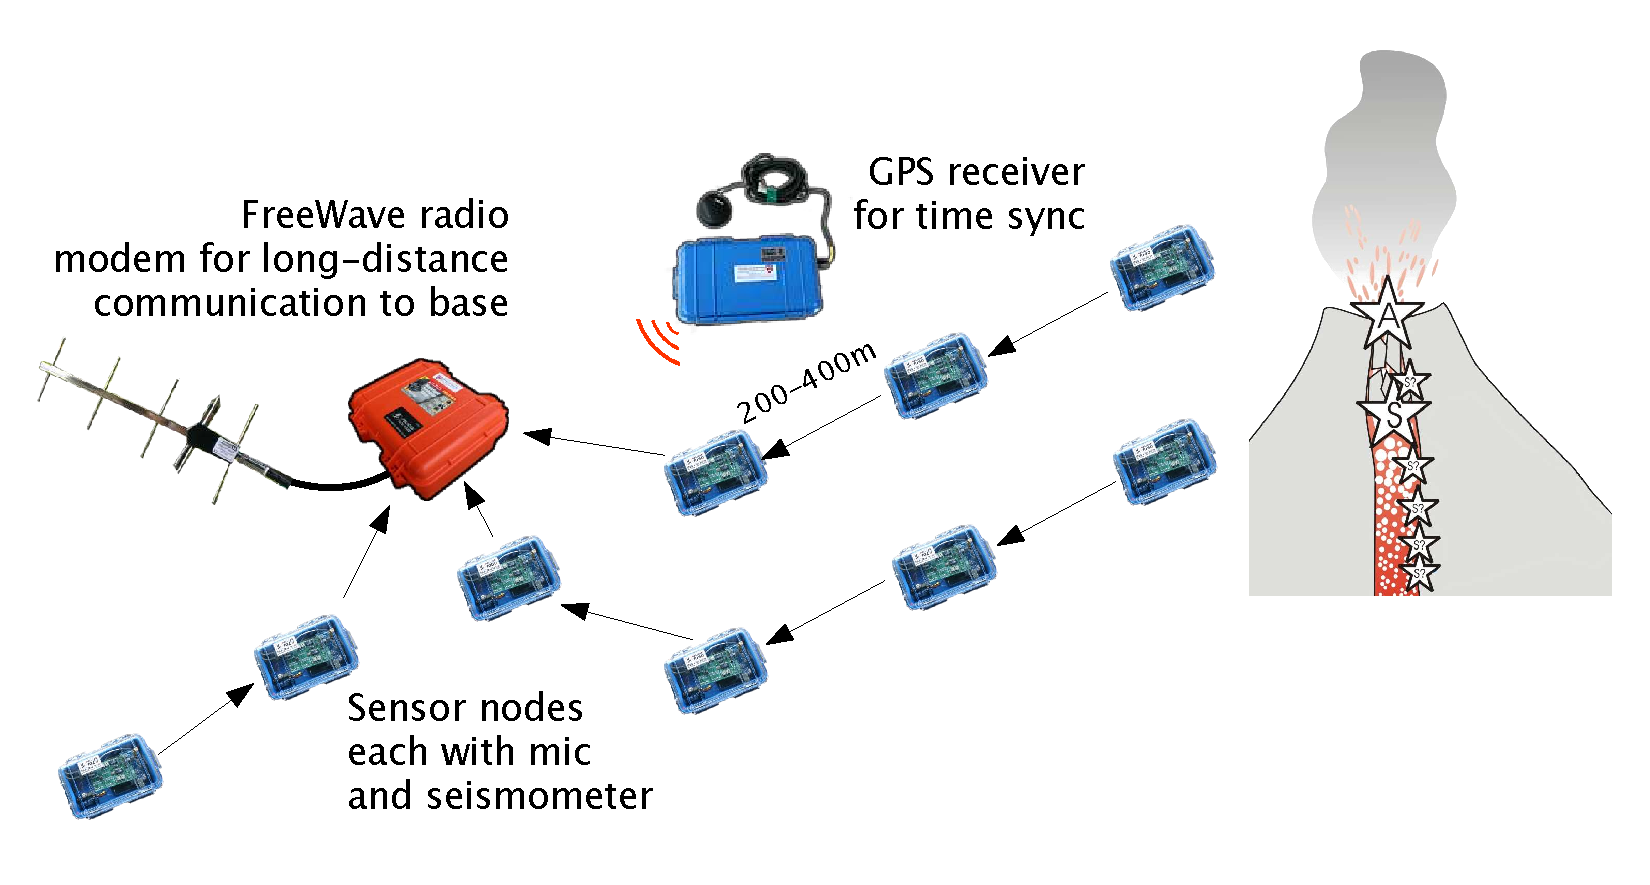
\includegraphics[width=1.0\hsize]{./3-evaluation/figs/schematic.pdf}
\end{center}
\caption{\textbf{Sensor network architecture.} Nodes form a multihop routing
topology, relaying data via a long-distance radio modem to the observatory. A
GPS receiver is used to establish a global timebase. The network topology
shown here was used during our deployment at Reventador.}
\label{evaluation-fig-schematic}
\end{figure}

\begin{figure}[t]
\begin{center}
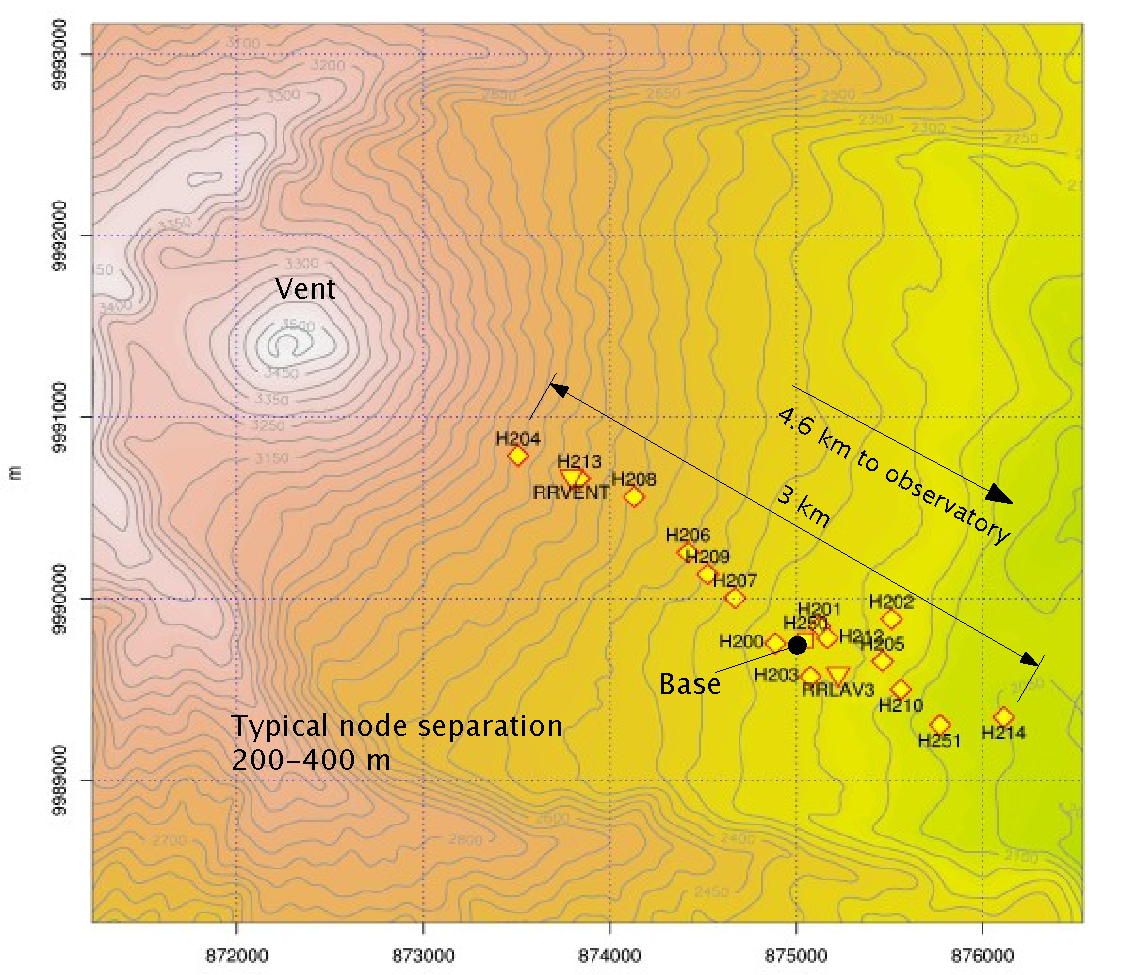
\includegraphics[width=0.8\hsize]{./3-evaluation/figs/map.pdf}
\end{center}
\caption{\textbf{2005 deployment location.} The figure shows the location of
our second volcano deployment in 2005: 16 nodes deployed on Reventador
Volcano.}
\label{evaluation-fig-map}
\end{figure}

We deployed 16~sensor nodes on the upper flanks of Reventador, as shown in
Figure~\ref{evaluation-fig-map}. The resulting multihop topology is shown in
Figure~\ref{evaluation-fig-schematic}. In addition to the sensor nodes, two
standalone seismic stations, consisting of a broadband sensor, a Reftek 130
data logger with 1~GByte flash memory cards, and a GPS receiver for
timestamping, were colocated with sensor nodes. The data from these stations
was critical for our network evaluation, as described in
Section~\ref{evaluation-sec-fidelity}.

We installed our stations in a roughly linear configuration, radiating away
from the vent and producing an aperture of over 3~km. We attempted to
position the stations as far apart as the radios on each node would allow.
Although our antennas could maintain radio links of over 400~m, the geography
at the deployment site occasionally required installing additional stations
to maintain radio connectivity. Other times we would deploy a node expecting
it to communicate with an immediate neighbor but later notice that that node
was bypassing its closest companion in favor of a node closer to the base
station. Most nodes communicated with the base station over three or fewer
hops, but a few were moving data over as many as six.
